% Created 2023-05-12 Fri 18:49
% Intended LaTeX compiler: pdflatex
\documentclass[bigger]{beamer}
\usepackage[utf8]{inputenc}
\usepackage[T1]{fontenc}
\usepackage{graphicx}
\usepackage{longtable}
\usepackage{wrapfig}
\usepackage{rotating}
\usepackage[normalem]{ulem}
\usepackage{amsmath}
\usepackage{amssymb}
\usepackage{capt-of}
\usepackage{hyperref}
\usepackage{amsfonts}
\usepackage{amsthm}
\usepackage{paralist}
\usepackage{bibunits}
\usepackage{xcolor}
\usepackage{natbib}
\usepackage{graphicx}
\usepackage{amsmath}
\usepackage{xcolor}
\usetheme{default}
\author{Yi Zhang}
\date{\textit{<2023-05-26 Fri>}}
\title{ODE parameter estimation in drug research: a deep dive into a Bayesian inference engine}
\AtBeginSection[]{\begin{frame}<beamer>\frametitle{Table of contents}\tableofcontents[currentsection]\end{frame}}
\hypersetup{
 pdfauthor={Yi Zhang},
 pdftitle={ODE parameter estimation in drug research: a deep dive into a Bayesian inference engine},
 pdfkeywords={},
 pdfsubject={},
 pdfcreator={Emacs 28.1 (Org mode 9.5.2)},
 pdflang={English}}
\begin{document}

\maketitle
\begin{frame}{Outline}
\tableofcontents
\end{frame}


\begin{frame}[label={sec:org5ca9ab6}]{NOT to talk about}
\begin{columns}
\begin{column}{0.50\columnwidth}
\begin{center}
\includegraphics[width=0.9\textwidth]{./figure/dont_want_2.jpg}
\end{center}
\end{column}


\begin{column}{0.50\columnwidth}
\begin{center}
\includegraphics[width=0.9\textwidth]{./figure/dont_want_3.jpg}
\end{center}
\end{column}
\end{columns}
\end{frame}


\section{The problem}
\label{sec:orgd4c792a}
\begin{frame}[label={sec:org6acaf57}]{Pharmacokinetics (PK) data}
\begin{figure}[htbp]
\centering
\includegraphics[width=0.9\textwidth]{./figure/twocpt_ppc_4x8.pdf}
\caption{Subject plasma concentration history (q12hx14).}
\end{figure}
\end{frame}

\begin{frame}[label={sec:org2168790}]{A Pharmacokinetics (PK) model}
\begin{align*}
  \frac{\mathrm d \hat{y}_\mathrm{gut}}{\mathrm d t} & = - k_a \hat{y}_\mathrm{gut} \\
  \frac{\mathrm d \hat{y}_\mathrm{cent}}{\mathrm d t} & = k_a \hat{y}_\mathrm{gut} -\left (k_{\text{CL}} + k_{\text{Q,cent}} \right) \hat{y}_\mathrm{cent} + k_{\text{Q,peri}} \hat{y}_\mathrm{peri} \\
  \frac{\mathrm d \hat{y}_\mathrm{peri}}{\mathrm d t} & = k_{\text{Q,cent}} \hat{y}_\mathrm{cent} - k_{\text{Q,peri}} \hat{y}_\mathrm{peri}
\end{align*}

\begin{center}
\includegraphics[width=0.6\textwidth]{./figure/TwoCptNice.png}
\end{center}
\end{frame}

\begin{frame}[label={sec:org1397c4e}]{A statistical model}
\begin{align*}
\theta & \equiv \{k_a, k_{\text{CL}}, k_{\text{Q,}\cdot}\},\\
\hat{y}(t) & = \hat{y}(t;\theta),\\
y(t) &\sim \text{Normal}(\hat{y}(t;\theta), \sigma).
\end{align*}

\begin{itemize}
\item play mix \& match with two models
\item Likelihood \(p(y | \theta)\).
\item Usually likelihood \(p(y | \theta, \sigma)\)
\end{itemize}
\end{frame}

\begin{frame}[label={sec:org80a232c}]{Estimate \(\theta\)}
\begin{itemize}
\item Maximum likelihood estimation
\(\theta_{\text{argmax}}(p(y|\theta))\)
\item Posterior distribution
\begin{align*}
  p(\theta | y) &= \frac{p(y|\theta)p(\theta)}{\bigcirc}\\
  \log{p(\theta|y)} &= C + \log{p(y | \theta)} + \log{p(\theta)}
\end{align*}
\item Connection to regularization
\end{itemize}
\end{frame}

\begin{frame}[label={sec:org2aa1a9f}]{Prior \& likelihood}
\begin{align*}
  \log{p(\theta|y)} &= C + \log{p(y | \theta)} + \log{p(\theta)}
\end{align*}
\begin{center}
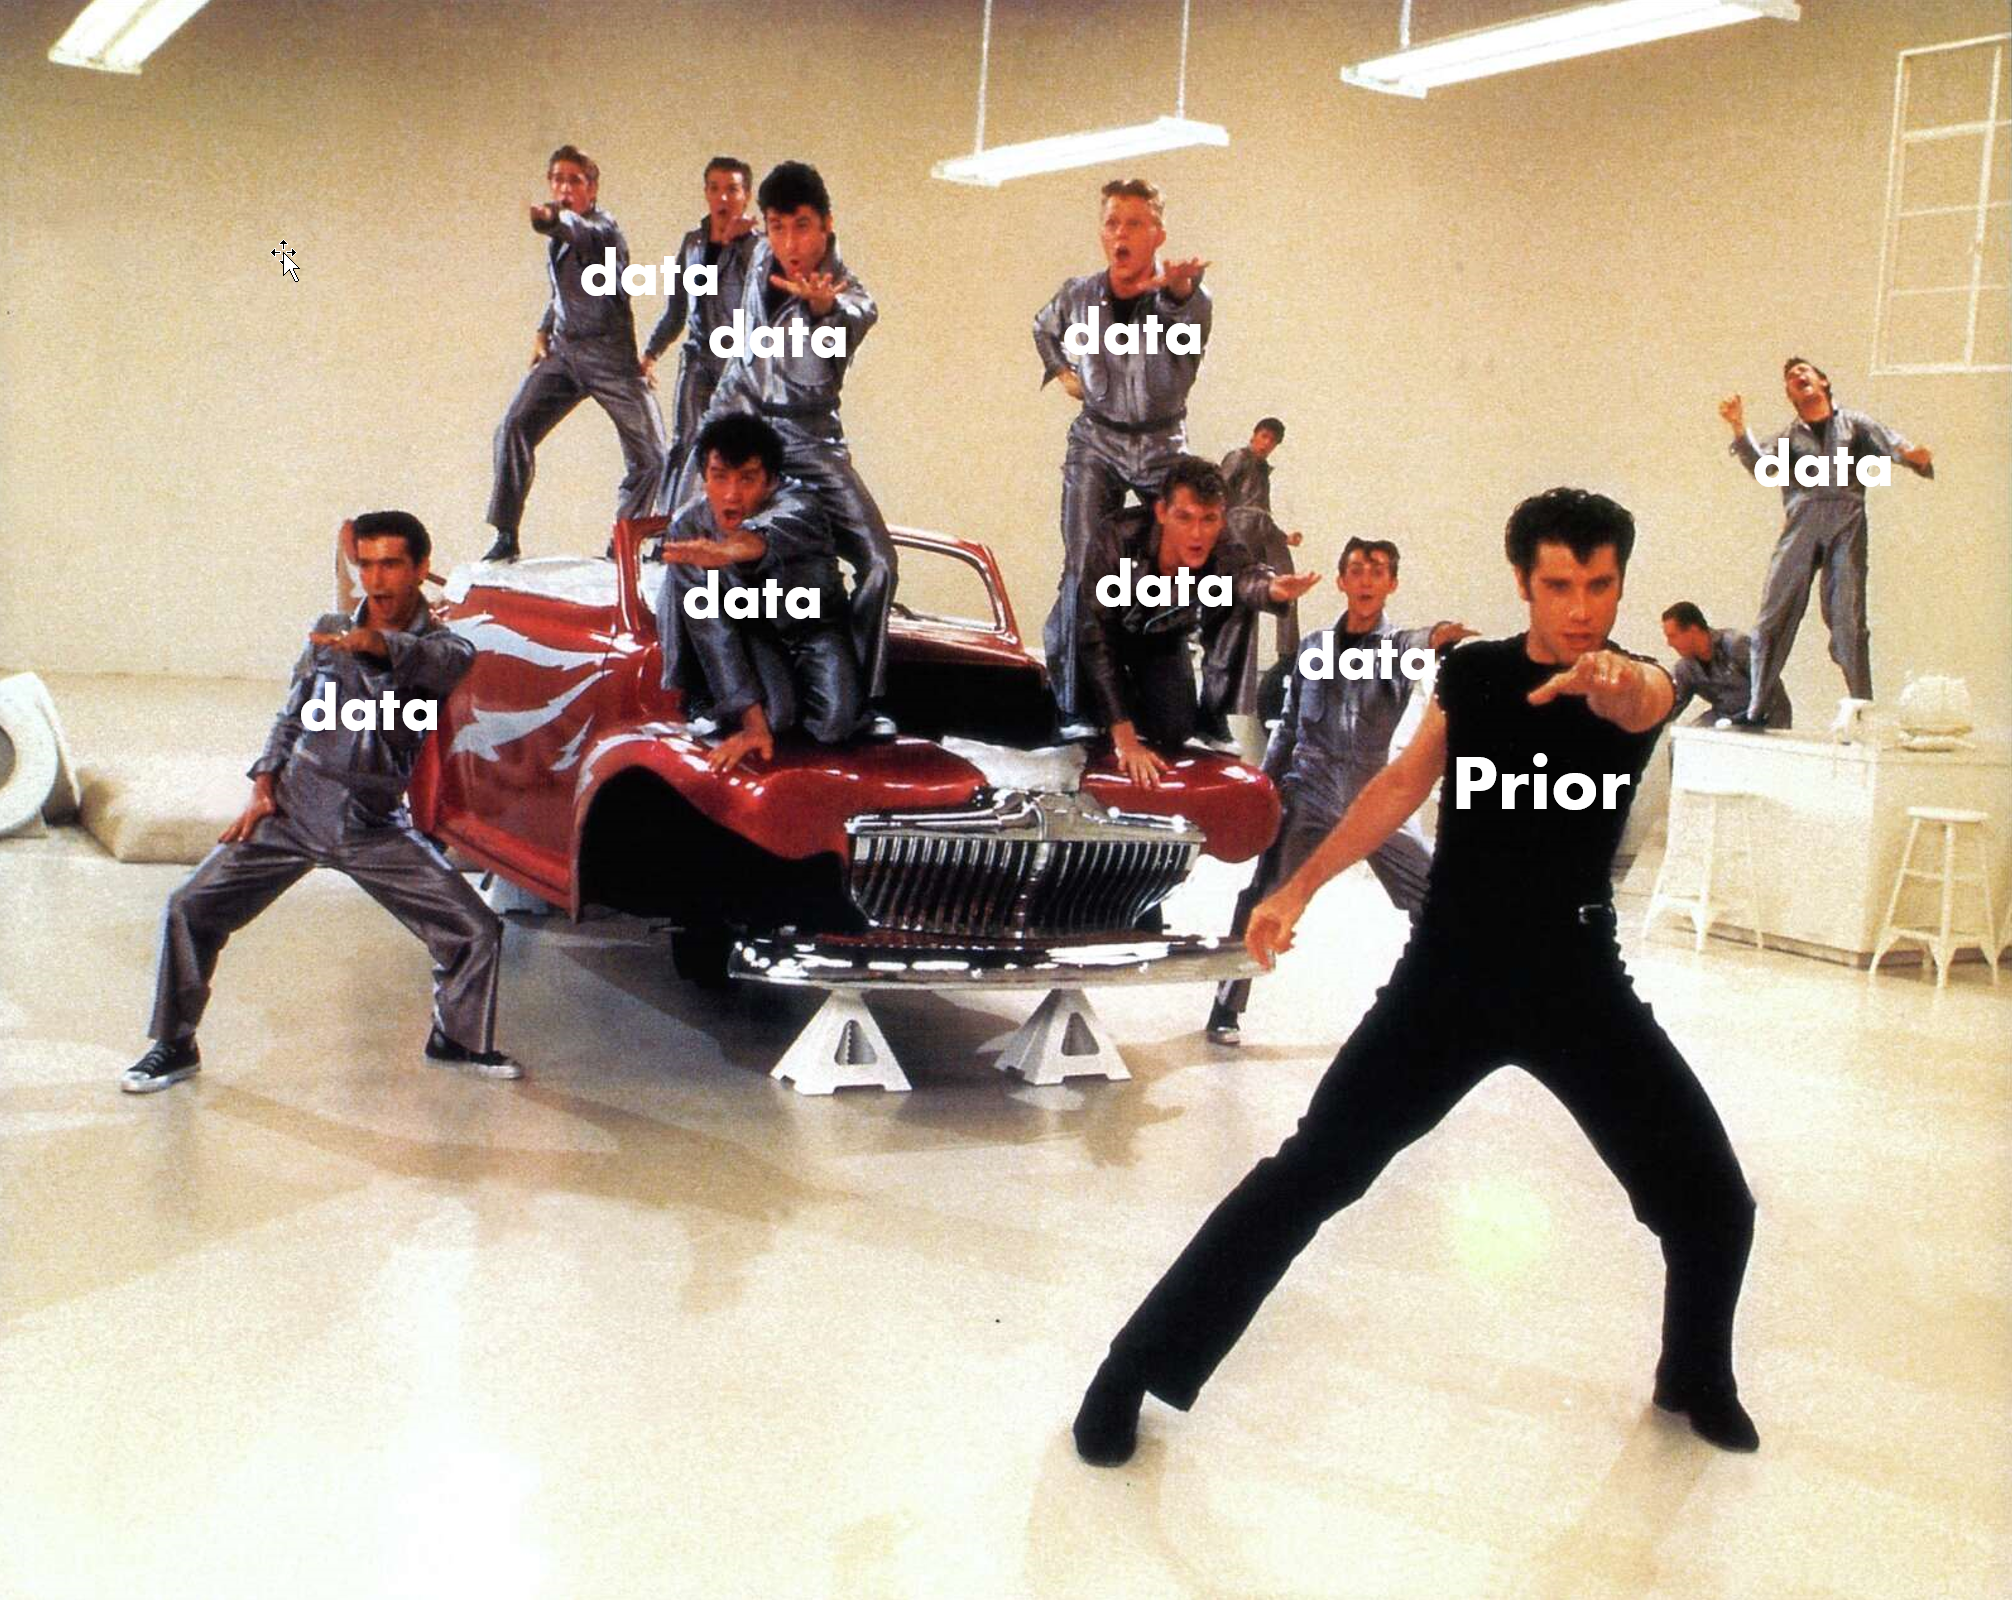
\includegraphics[width=0.7\textwidth]{./figure/prior_and_data.png}
\end{center}
\end{frame}


\begin{frame}[label={sec:org40c9c6d}]{Sample the posterior}
\(\text{target (distribution)} = \log{p(\theta|y)} = \log{p(y | \theta)} + \log{p(\theta)}\)

\begin{itemize}
\item <1-> Posterior from an oracle: \(\theta \rightarrow \log{p(\theta | y)}\)
\item <2-> Every query costs one ODE solution
\item <3-> Sampling procedure for a distribution: \(\theta^{(1)}, \theta^{(2)}, \dots\)
\begin{equation*}
  \lim_{n\rightarrow }\frac{1}{n}\sum{f(\theta^{(i)})}=\mathbb{E}(f)
\end{equation*}
\item <4-> MCMC: \(p(\theta^{(i)} | y, \theta^{(i-1)},  \theta^{(i-2)}, \dots, \theta^{(1)})=p(\theta^{(i)} | y, \theta^{(i-1)})\)
\end{itemize}
\end{frame}

\begin{frame}[label={sec:org6aa4db4}]{The Metropolis-Hastings algorithm}
Proposal-rejection from \(\theta^{(i)}\) to \(\theta^{(i+1)}\).
\begin{enumerate}
\item Propose \(\theta^{(i+1)}\) according to transition density \(q(\theta^{(i+1)}, \theta^{(i)})\).
\item Accept \(\theta^{(i+1)}\) with probability
\end{enumerate}
\begin{equation}
  \alpha(\theta^{(i)}, \theta^{(i+1)}) = \min\left[
    1, \frac{p(\theta^{(i+1)}|y)q(\theta^{(i)}, \theta^{(i+1)})}{p(\theta^{(i)}|y)q(\theta^{(i+1)}, \theta^{(i)})}
    \right]
\end{equation}
otherwise reject.

\begin{itemize}
\item Chain generated by M-H has detailed balance with \(p(\theta|y)\) as
its stationary distribution.
\item Convergence in TVD with proper proposal that garantees irreducibility.
\end{itemize}
\end{frame}

\begin{frame}[label={sec:orgdbeeb5d}]{Why MCMC?}
\begin{quote}
Monte Carlo is an extremely bad method; it should be used only when all alternative methods
are worse.
-- Sokal, A. D. (1989). "Monte carlo methods in statistical mechanics: foundations and new algorithms."
\end{quote}
\begin{center}
\includegraphics[width=0.7\textwidth]{./figure/simply_not_mcmc.jpg}
\end{center}
\end{frame}


\section{You're Gonna Need a Bigger Boat}
\label{sec:orge4b6bb2}
\begin{frame}[label={sec:orgc17fb33}]{The problem}
\begin{center}
\includegraphics[width=\textwidth]{./figure/twocpt_pop_ppc1.pdf}
\end{center}
\end{frame}

\begin{frame}[label={sec:orgdde934a}]{Hierarchical model}
\begin{columns}
\begin{column}{0.4\columnwidth}
\begin{align*}
\theta_0 &\sim \text{Prior}(\cdot),\\
\theta_i &\sim \text{MultiNormal}(\theta_0, \Sigma),\\
y_i &\sim \text{Normal}(\hat{y}_i(\theta_i), \sigma),\\
\theta &= \{\theta_0, \theta_1, \dots, \theta_n, \sigma\}
\end{align*}
\end{column}

\begin{column}{0.6\columnwidth}
\begin{itemize}
\item <1-> Posterior(likelihood) equation is an oracle
\item <2-> Curse of dimensionality
\begin{itemize}
\item <2-> Computational tractability
\item <3-> Concentration of measure (e.g. high dimensional gaussian distribution is like uniform distribution)
\end{itemize}
\item <4-> Geometry of posterior
\end{itemize}
\end{column}
\end{columns}
\end{frame}

\begin{frame}[label={sec:orga2abadd}]{Challenges: high dimensional gaussian distribution}
\(p(|\|y_d\|_2-\sqrt{d}| \ge t) \le 2\exp{(-ct^2)}, \forall t\ge 0\).
\begin{columns}
\begin{column}{0.5\columnwidth}
\begin{figure}[htbp]
\centering
\includegraphics[width=0.8\textwidth]{./figure/high_dim_gaussian.png}
\caption{\(\|y_d\|_2, y_d \sim \text{Normal}(0, \mathbb{I}_d)\)}
\end{figure}

Average is not representative.
Random Walk sampler is not efficient.
\end{column}

\begin{column}{0.5\columnwidth}
\begin{center}
\includegraphics[width=0.6\textwidth]{./figure/d2_normal_point.png}
\end{center}

\begin{center}
\includegraphics[width=0.6\textwidth]{./figure/d100_normal_point.png}
\end{center}
\end{column}
\end{columns}
\end{frame}

\begin{frame}[label={sec:org1efa3a8}]{Challenges: Geometry of posterior}
\begin{columns}
\begin{column}{0.4\columnwidth}
\begin{align*}
  \theta_0 &= 0,\\
  \kappa &\sim \text{Normal}(0, 3),\\
  \theta_i(k) &\sim \text{Normal}(0, \exp{(\kappa/2)}),\\
  k&=1,2,\dots
\end{align*}
\end{column}

\begin{column}{0.6\columnwidth}
\begin{figure}[htbp]
\centering
\includegraphics[width=\textwidth]{./figure/funnel.png}
\caption{Neal's funnel}
\end{figure}
Mode is not representative.
Optimizer is not efficient.
\end{column}
\end{columns}
\end{frame}

\section{Up In the Air}
\label{sec:org2ff9ada}
\begin{frame}[label={sec:orgee332a0}]{Hamiltonian Monte Carlo}
\begin{align*}
  H(\theta, r) &= -\log{p(r, \theta | y)} = T(r) + V(\theta) = -\log{r} - \log{p(\theta|y)},\\
  \frac{d\theta}{dt} &= \frac{\partial H}{\partial r},\qquad
  \frac{dr}{dt} = -\frac{\partial H}{\partial \theta},
\end{align*}
\begin{columns}
\begin{column}{0.5\columnwidth}
\begin{center}
\includegraphics[width=0.8\textwidth]{./figure/d2_normal_point.png}
\end{center}
\end{column}

\begin{column}{0.5\columnwidth}
\begin{center}
\includegraphics[width=0.8\textwidth]{./figure/d100_normal_point.png}
\end{center}
\end{column}
\end{columns}
\end{frame}


\begin{frame}[label={sec:org1e0b244}]{Hamiltonian Monte Carlo}
\begin{align*}
  H(\theta, r) &= -\log{p(r, \theta | y)} = T(r) + V(\theta) = -\log{r} - \log{p(\theta|y)},\\
  \frac{d\theta}{dt} &= \frac{\partial H}{\partial r},\qquad
  \frac{dr}{dt} = -\frac{\partial H}{\partial \theta},
\end{align*}
Apply M-H to \(p(r, \theta)\)
\begin{align*}
  \alpha((r^{(i)}, \theta^{(i)}), (r^{(i+1)}, \theta^{(i+1)})) &= \min\left[
    1, \frac{p(r^{(i+1)}, \theta^{(i+1)}|y)q()}{p(r^{(i)}, \theta^{(i)}|y)q()}
  \right]\\
  &= \min\left[
    1, \frac{p(r^{(i+1)}, \theta^{(i+1)}|y)}{p(r^{(i)}, \theta^{(i)}|y)}
  \right]
\end{align*}
\begin{equation*}
  \alpha(\cdot, \cdot) =\min\left[
    1, \exp{(H(\theta^{(i)}, r^{(i)}) - H(\theta^{(i+1)}, r^{(i+1)}))}
  \right]
\end{equation*}
\end{frame}


\begin{frame}[label={sec:org0a478d4}]{Hamiltonian Monte Carlo}
\begin{equation*}
  p(\theta^{(i)} \rightarrow \theta^{(i+1)}) =\min\left[
    1, \exp{(H(\theta^{(i)}, r^{(i)}) - H(\theta^{(i+1)}, r^{(i+1)}))}
  \right]
\end{equation*}
Proposal \((r^{(i+1)}, \theta^{(i+1)})\):
\begin{align*}
  r \sim \text{Normal}(0, M),\\
  (r^{(i)}, \theta^{(i)}) \rightarrow (r^{(i+1)}, \theta^{(i+1)})
\end{align*}
\end{frame}


\begin{frame}[label={sec:orgb1c3ccd}]{A principled sampler for \(p(\theta|y)\)}
\begin{columns}
\begin{column}{0.8\columnwidth}
\begin{center}
\includegraphics[width=0.9\textwidth]{./figure/sampler_path.png}
\end{center}
\end{column}

\begin{column}{0.2\columnwidth}
\begin{center}
\includegraphics[width=0.7\textwidth]{./figure/sampler_path2.png}
\end{center}
\end{column}
\end{columns}
\end{frame}


\section{Small moves, Ellie. Small moves}
\label{sec:org7d224d2}
\begin{frame}[label={sec:org066842c}]{A tale of two ODEs}
\(\theta\)\textsuperscript{(i)} = \{\(\theta\)\textsuperscript{(i)}\textsubscript{j}\}, j=1,2,\dots{},n: \((r, \theta)(\tau^{(i)}) \rightarrow (r, \theta)(\tau^{(i+1)})\)
\begin{align*}
\begin{cases}
  &\theta^{(i)}_j \rightarrow \hat{y}_j(t; \theta^{(i)}_j),\\
  &y_{jk} \sim \text{Normal}(\hat{y}_{jk}(\theta_j), \sigma),\quad p(y_{jk}|\theta_j) = \frac{1}{\sigma\sqrt{2\pi}}\exp{\left[-\frac{(\hat{y}_{jk}(\theta_j)-y_{jk})^2}{2\sigma^2}\right]}
\end{cases}
\end{align*}
Nested ODE solvers:
\begin{align*}
  r^{(i+1/2)} &= r^{(i)} - \frac{h}{2}\nabla_{\theta} \log{p(\theta^{(i)} | y)},\text{  a step in leapfrog}\\
  \nabla_{\theta} \log{p(\theta^{(i)} | y)} &= \nabla_{\theta} \log{p(\theta^{(i)})} + \nabla_{\theta} \log{p(y | \theta^{(i)})},\\
  \nabla_{\theta} \log{p(y | \theta^{(i)})} &= - (\cdots)\sum_{j,k}\nabla_{\theta} \frac{\hat{y}_{jk}(\theta_j^{(i)}) - y_{jk}}{\sigma^{(i)}} + \dots
\end{align*}
\end{frame}

\begin{frame}[label={sec:org7ca33d2}]{Automatic differentiation (1 obsv/subject: k=1)}
\begin{center}
\includegraphics[width=\textwidth]{./figure/autodiff_diag.pdf}
\end{center}
\end{frame}

\begin{frame}[label={sec:org86fe9c3}]{Automatic differentiation}
\begin{columns}
\begin{column}{0.5\columnwidth}
\begin{center}
\includegraphics[width=0.7\textwidth]{./figure/stan_single_funcs.png}
\end{center}
\end{column}

\begin{column}{0.5\columnwidth}
\begin{center}
\includegraphics[width=0.9\textwidth]{./figure/everyone_adjoint.jpg}
\end{center}
\end{column}
\end{columns}
\end{frame}

\begin{frame}[label={sec:orgb084b0e}]{Sensitivity solution}
\begin{align*}
  &\frac{d\hat{y}}{dt} = f(t, \hat{y};\theta) \rightarrow \nabla_{\theta} \frac{d\hat{y}}{dt} = \nabla_{\theta} f(t, \hat{y};\theta)\\
  &\frac{d\nabla_{\theta} \hat{y}}{dt} = f_{\theta} + f_{\hat{y}}\nabla_{\theta}\hat{y}
\end{align*}
Use the autodiff calculate \(f_{\theta}\) and \(f_{\hat{y}}\).
\end{frame}



\begin{frame}[label={sec:orgc79e445}]{Estimation}
\begin{center}
\includegraphics[width=\textwidth]{./figure/pop_trace.pdf}
\end{center}
\end{frame}

\begin{frame}[label={sec:orgd4661f4}]{Estimation}
\begin{center}
\includegraphics[width=\textwidth]{./figure/pop_dens.pdf}
\end{center}
\end{frame}


\begin{frame}[label={sec:orgfebfa9c}]{Misc}
\begin{itemize}
\item Diagnostics
\item Parallel chains
\item Within-chain parallellization
\end{itemize}
\end{frame}
\end{document}